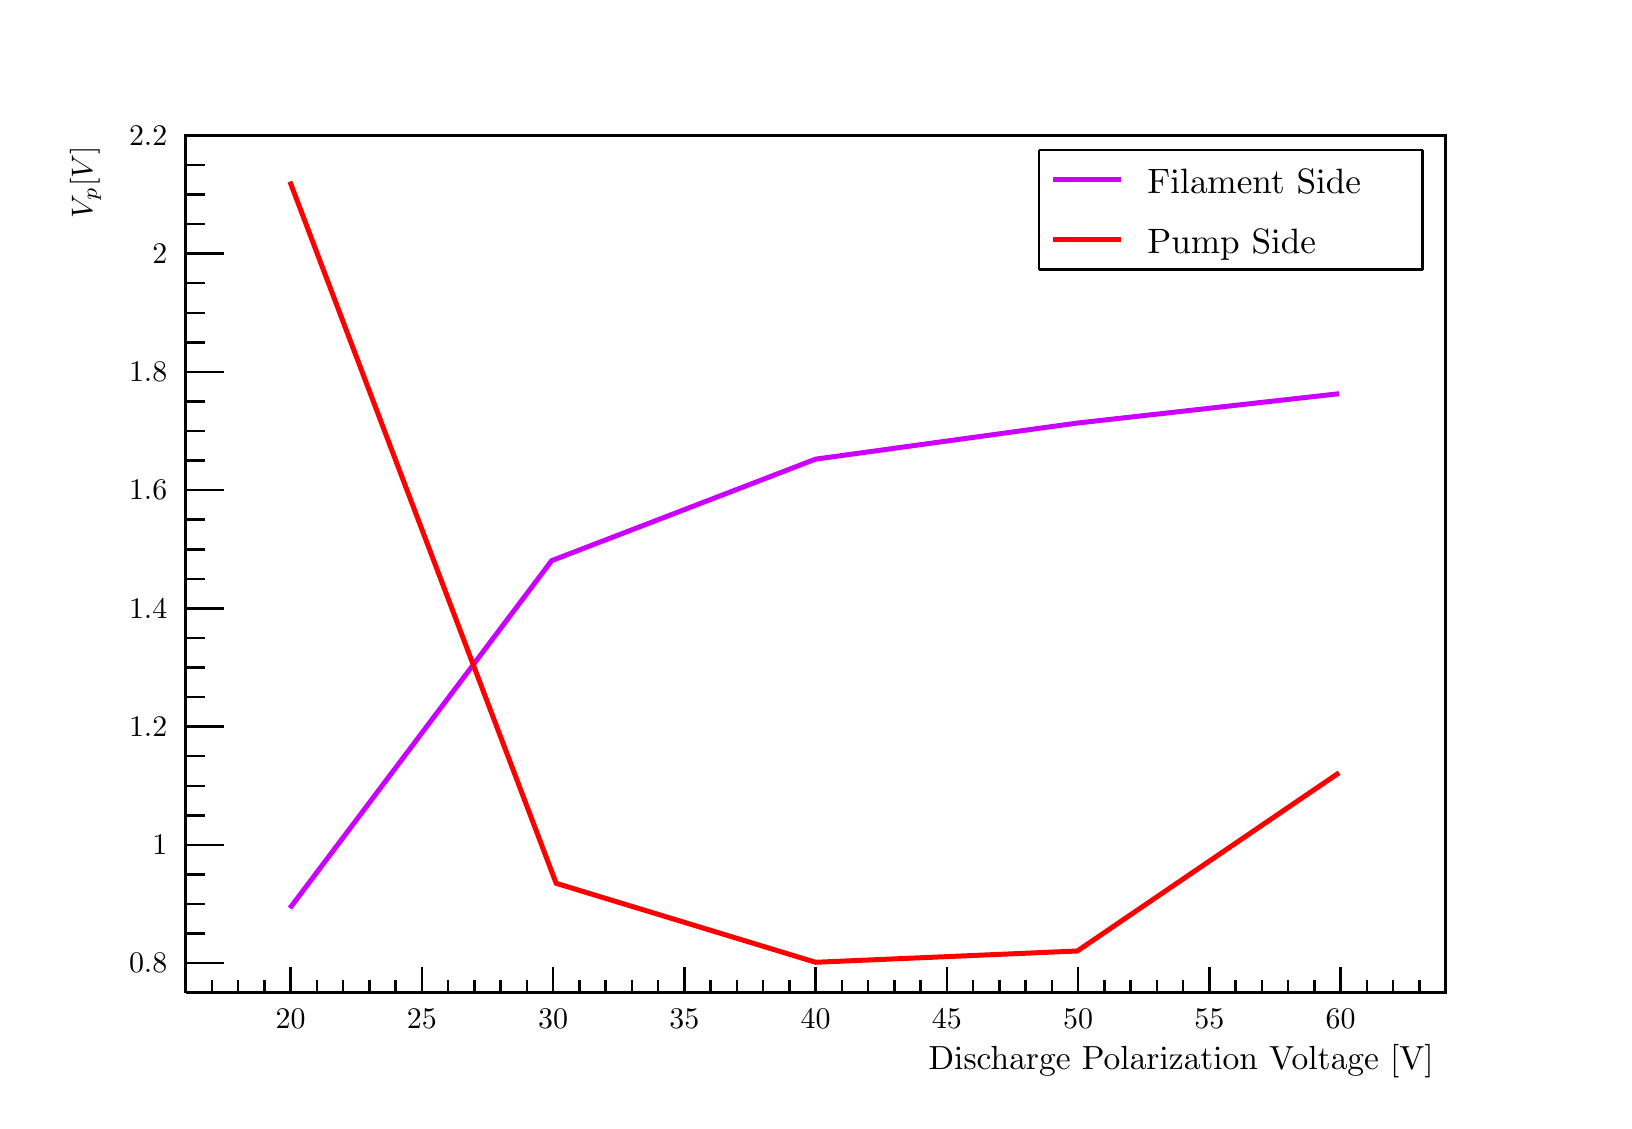
\begin{tikzpicture}
\pgfdeclareplotmark{cross} {
\pgfpathmoveto{\pgfpoint{-0.3\pgfplotmarksize}{\pgfplotmarksize}}
\pgfpathlineto{\pgfpoint{+0.3\pgfplotmarksize}{\pgfplotmarksize}}
\pgfpathlineto{\pgfpoint{+0.3\pgfplotmarksize}{0.3\pgfplotmarksize}}
\pgfpathlineto{\pgfpoint{+1\pgfplotmarksize}{0.3\pgfplotmarksize}}
\pgfpathlineto{\pgfpoint{+1\pgfplotmarksize}{-0.3\pgfplotmarksize}}
\pgfpathlineto{\pgfpoint{+0.3\pgfplotmarksize}{-0.3\pgfplotmarksize}}
\pgfpathlineto{\pgfpoint{+0.3\pgfplotmarksize}{-1.\pgfplotmarksize}}
\pgfpathlineto{\pgfpoint{-0.3\pgfplotmarksize}{-1.\pgfplotmarksize}}
\pgfpathlineto{\pgfpoint{-0.3\pgfplotmarksize}{-0.3\pgfplotmarksize}}
\pgfpathlineto{\pgfpoint{-1.\pgfplotmarksize}{-0.3\pgfplotmarksize}}
\pgfpathlineto{\pgfpoint{-1.\pgfplotmarksize}{0.3\pgfplotmarksize}}
\pgfpathlineto{\pgfpoint{-0.3\pgfplotmarksize}{0.3\pgfplotmarksize}}
\pgfpathclose
\pgfusepathqstroke
}
\pgfdeclareplotmark{cross*} {
\pgfpathmoveto{\pgfpoint{-0.3\pgfplotmarksize}{\pgfplotmarksize}}
\pgfpathlineto{\pgfpoint{+0.3\pgfplotmarksize}{\pgfplotmarksize}}
\pgfpathlineto{\pgfpoint{+0.3\pgfplotmarksize}{0.3\pgfplotmarksize}}
\pgfpathlineto{\pgfpoint{+1\pgfplotmarksize}{0.3\pgfplotmarksize}}
\pgfpathlineto{\pgfpoint{+1\pgfplotmarksize}{-0.3\pgfplotmarksize}}
\pgfpathlineto{\pgfpoint{+0.3\pgfplotmarksize}{-0.3\pgfplotmarksize}}
\pgfpathlineto{\pgfpoint{+0.3\pgfplotmarksize}{-1.\pgfplotmarksize}}
\pgfpathlineto{\pgfpoint{-0.3\pgfplotmarksize}{-1.\pgfplotmarksize}}
\pgfpathlineto{\pgfpoint{-0.3\pgfplotmarksize}{-0.3\pgfplotmarksize}}
\pgfpathlineto{\pgfpoint{-1.\pgfplotmarksize}{-0.3\pgfplotmarksize}}
\pgfpathlineto{\pgfpoint{-1.\pgfplotmarksize}{0.3\pgfplotmarksize}}
\pgfpathlineto{\pgfpoint{-0.3\pgfplotmarksize}{0.3\pgfplotmarksize}}
\pgfpathclose
\pgfusepathqfillstroke
}
\pgfdeclareplotmark{newstar} {
\pgfpathmoveto{\pgfqpoint{0pt}{\pgfplotmarksize}}
\pgfpathlineto{\pgfqpointpolar{44}{0.5\pgfplotmarksize}}
\pgfpathlineto{\pgfqpointpolar{18}{\pgfplotmarksize}}
\pgfpathlineto{\pgfqpointpolar{-20}{0.5\pgfplotmarksize}}
\pgfpathlineto{\pgfqpointpolar{-54}{\pgfplotmarksize}}
\pgfpathlineto{\pgfqpointpolar{-90}{0.5\pgfplotmarksize}}
\pgfpathlineto{\pgfqpointpolar{234}{\pgfplotmarksize}}
\pgfpathlineto{\pgfqpointpolar{198}{0.5\pgfplotmarksize}}
\pgfpathlineto{\pgfqpointpolar{162}{\pgfplotmarksize}}
\pgfpathlineto{\pgfqpointpolar{134}{0.5\pgfplotmarksize}}
\pgfpathclose
\pgfusepathqstroke
}
\pgfdeclareplotmark{newstar*} {
\pgfpathmoveto{\pgfqpoint{0pt}{\pgfplotmarksize}}
\pgfpathlineto{\pgfqpointpolar{44}{0.5\pgfplotmarksize}}
\pgfpathlineto{\pgfqpointpolar{18}{\pgfplotmarksize}}
\pgfpathlineto{\pgfqpointpolar{-20}{0.5\pgfplotmarksize}}
\pgfpathlineto{\pgfqpointpolar{-54}{\pgfplotmarksize}}
\pgfpathlineto{\pgfqpointpolar{-90}{0.5\pgfplotmarksize}}
\pgfpathlineto{\pgfqpointpolar{234}{\pgfplotmarksize}}
\pgfpathlineto{\pgfqpointpolar{198}{0.5\pgfplotmarksize}}
\pgfpathlineto{\pgfqpointpolar{162}{\pgfplotmarksize}}
\pgfpathlineto{\pgfqpointpolar{134}{0.5\pgfplotmarksize}}
\pgfpathclose
\pgfusepathqfillstroke
}
\definecolor{c}{rgb}{1,1,1};
\draw [color=c, fill=c] (0,0) rectangle (20,13.6103);
\draw [color=c, fill=c] (2,1.36103) rectangle (18,12.2493);
\definecolor{c}{rgb}{0,0,0};
\draw [c,line width=0.9] (2,1.36103) -- (2,12.2493) -- (18,12.2493) -- (18,1.36103) -- (2,1.36103);
\definecolor{c}{rgb}{1,1,1};
\draw [color=c, fill=c] (2,1.36103) rectangle (18,12.2493);
\definecolor{c}{rgb}{0,0,0};
\draw [c,line width=0.9] (2,1.36103) -- (2,12.2493) -- (18,12.2493) -- (18,1.36103) -- (2,1.36103);
\draw [c,line width=0.9] (2,1.36103) -- (18,1.36103);
\draw [c,line width=0.9] (3.33333,1.68768) -- (3.33333,1.36103);
\draw [c,line width=0.9] (3.66667,1.52436) -- (3.66667,1.36103);
\draw [c,line width=0.9] (4,1.52436) -- (4,1.36103);
\draw [c,line width=0.9] (4.33333,1.52436) -- (4.33333,1.36103);
\draw [c,line width=0.9] (4.66667,1.52436) -- (4.66667,1.36103);
\draw [c,line width=0.9] (5,1.68768) -- (5,1.36103);
\draw [c,line width=0.9] (5.33333,1.52436) -- (5.33333,1.36103);
\draw [c,line width=0.9] (5.66667,1.52436) -- (5.66667,1.36103);
\draw [c,line width=0.9] (6,1.52436) -- (6,1.36103);
\draw [c,line width=0.9] (6.33333,1.52436) -- (6.33333,1.36103);
\draw [c,line width=0.9] (6.66667,1.68768) -- (6.66667,1.36103);
\draw [c,line width=0.9] (7,1.52436) -- (7,1.36103);
\draw [c,line width=0.9] (7.33333,1.52436) -- (7.33333,1.36103);
\draw [c,line width=0.9] (7.66667,1.52436) -- (7.66667,1.36103);
\draw [c,line width=0.9] (8,1.52436) -- (8,1.36103);
\draw [c,line width=0.9] (8.33333,1.68768) -- (8.33333,1.36103);
\draw [c,line width=0.9] (8.66667,1.52436) -- (8.66667,1.36103);
\draw [c,line width=0.9] (9,1.52436) -- (9,1.36103);
\draw [c,line width=0.9] (9.33333,1.52436) -- (9.33333,1.36103);
\draw [c,line width=0.9] (9.66667,1.52436) -- (9.66667,1.36103);
\draw [c,line width=0.9] (10,1.68768) -- (10,1.36103);
\draw [c,line width=0.9] (10.3333,1.52436) -- (10.3333,1.36103);
\draw [c,line width=0.9] (10.6667,1.52436) -- (10.6667,1.36103);
\draw [c,line width=0.9] (11,1.52436) -- (11,1.36103);
\draw [c,line width=0.9] (11.3333,1.52436) -- (11.3333,1.36103);
\draw [c,line width=0.9] (11.6667,1.68768) -- (11.6667,1.36103);
\draw [c,line width=0.9] (12,1.52436) -- (12,1.36103);
\draw [c,line width=0.9] (12.3333,1.52436) -- (12.3333,1.36103);
\draw [c,line width=0.9] (12.6667,1.52436) -- (12.6667,1.36103);
\draw [c,line width=0.9] (13,1.52436) -- (13,1.36103);
\draw [c,line width=0.9] (13.3333,1.68768) -- (13.3333,1.36103);
\draw [c,line width=0.9] (13.6667,1.52436) -- (13.6667,1.36103);
\draw [c,line width=0.9] (14,1.52436) -- (14,1.36103);
\draw [c,line width=0.9] (14.3333,1.52436) -- (14.3333,1.36103);
\draw [c,line width=0.9] (14.6667,1.52436) -- (14.6667,1.36103);
\draw [c,line width=0.9] (15,1.68768) -- (15,1.36103);
\draw [c,line width=0.9] (15.3333,1.52436) -- (15.3333,1.36103);
\draw [c,line width=0.9] (15.6667,1.52436) -- (15.6667,1.36103);
\draw [c,line width=0.9] (16,1.52436) -- (16,1.36103);
\draw [c,line width=0.9] (16.3333,1.52436) -- (16.3333,1.36103);
\draw [c,line width=0.9] (16.6667,1.68768) -- (16.6667,1.36103);
\draw [c,line width=0.9] (3.33333,1.68768) -- (3.33333,1.36103);
\draw [c,line width=0.9] (3,1.52436) -- (3,1.36103);
\draw [c,line width=0.9] (2.66667,1.52436) -- (2.66667,1.36103);
\draw [c,line width=0.9] (2.33333,1.52436) -- (2.33333,1.36103);
\draw [c,line width=0.9] (2,1.52436) -- (2,1.36103);
\draw [c,line width=0.9] (16.6667,1.68768) -- (16.6667,1.36103);
\draw [c,line width=0.9] (17,1.52436) -- (17,1.36103);
\draw [c,line width=0.9] (17.3333,1.52436) -- (17.3333,1.36103);
\draw [c,line width=0.9] (17.6667,1.52436) -- (17.6667,1.36103);
\draw [anchor=base] (3.33333,0.911891) node[scale=1.08185, color=c, rotate=0]{20};
\draw [anchor=base] (5,0.911891) node[scale=1.08185, color=c, rotate=0]{25};
\draw [anchor=base] (6.66667,0.911891) node[scale=1.08185, color=c, rotate=0]{30};
\draw [anchor=base] (8.33333,0.911891) node[scale=1.08185, color=c, rotate=0]{35};
\draw [anchor=base] (10,0.911891) node[scale=1.08185, color=c, rotate=0]{40};
\draw [anchor=base] (11.6667,0.911891) node[scale=1.08185, color=c, rotate=0]{45};
\draw [anchor=base] (13.3333,0.911891) node[scale=1.08185, color=c, rotate=0]{50};
\draw [anchor=base] (15,0.911891) node[scale=1.08185, color=c, rotate=0]{55};
\draw [anchor=base] (16.6667,0.911891) node[scale=1.08185, color=c, rotate=0]{60};
\draw [anchor= east] (18,0.489972) node[scale=1.20912, color=c, rotate=0]{Discharge Polarization Voltage [V]};
\draw [c,line width=0.9] (2,1.36103) -- (2,12.2493);
\draw [c,line width=0.9] (2.48,1.73649) -- (2,1.73649);
\draw [c,line width=0.9] (2.24,2.11195) -- (2,2.11195);
\draw [c,line width=0.9] (2.24,2.4874) -- (2,2.4874);
\draw [c,line width=0.9] (2.24,2.86286) -- (2,2.86286);
\draw [c,line width=0.9] (2.48,3.23832) -- (2,3.23832);
\draw [c,line width=0.9] (2.24,3.61377) -- (2,3.61377);
\draw [c,line width=0.9] (2.24,3.98923) -- (2,3.98923);
\draw [c,line width=0.9] (2.24,4.36469) -- (2,4.36469);
\draw [c,line width=0.9] (2.48,4.74014) -- (2,4.74014);
\draw [c,line width=0.9] (2.24,5.1156) -- (2,5.1156);
\draw [c,line width=0.9] (2.24,5.49106) -- (2,5.49106);
\draw [c,line width=0.9] (2.24,5.86652) -- (2,5.86652);
\draw [c,line width=0.9] (2.48,6.24197) -- (2,6.24197);
\draw [c,line width=0.9] (2.24,6.61743) -- (2,6.61743);
\draw [c,line width=0.9] (2.24,6.99289) -- (2,6.99289);
\draw [c,line width=0.9] (2.24,7.36834) -- (2,7.36834);
\draw [c,line width=0.9] (2.48,7.7438) -- (2,7.7438);
\draw [c,line width=0.9] (2.24,8.11926) -- (2,8.11926);
\draw [c,line width=0.9] (2.24,8.49471) -- (2,8.49471);
\draw [c,line width=0.9] (2.24,8.87017) -- (2,8.87017);
\draw [c,line width=0.9] (2.48,9.24563) -- (2,9.24563);
\draw [c,line width=0.9] (2.24,9.62109) -- (2,9.62109);
\draw [c,line width=0.9] (2.24,9.99654) -- (2,9.99654);
\draw [c,line width=0.9] (2.24,10.372) -- (2,10.372);
\draw [c,line width=0.9] (2.48,10.7475) -- (2,10.7475);
\draw [c,line width=0.9] (2.24,11.1229) -- (2,11.1229);
\draw [c,line width=0.9] (2.24,11.4984) -- (2,11.4984);
\draw [c,line width=0.9] (2.24,11.8738) -- (2,11.8738);
\draw [c,line width=0.9] (2.48,12.2493) -- (2,12.2493);
\draw [c,line width=0.9] (2.48,1.73649) -- (2,1.73649);
\draw [c,line width=0.9] (2.24,1.36103) -- (2,1.36103);
\draw [anchor= east] (1.9,1.73649) node[scale=1.08185, color=c, rotate=0]{0.8};
\draw [anchor= east] (1.9,3.23832) node[scale=1.08185, color=c, rotate=0]{1};
\draw [anchor= east] (1.9,4.74014) node[scale=1.08185, color=c, rotate=0]{1.2};
\draw [anchor= east] (1.9,6.24197) node[scale=1.08185, color=c, rotate=0]{1.4};
\draw [anchor= east] (1.9,7.7438) node[scale=1.08185, color=c, rotate=0]{1.6};
\draw [anchor= east] (1.9,9.24563) node[scale=1.08185, color=c, rotate=0]{1.8};
\draw [anchor= east] (1.9,10.7475) node[scale=1.08185, color=c, rotate=0]{2};
\draw [anchor= east] (1.9,12.2493) node[scale=1.08185, color=c, rotate=0]{2.2};
\draw [anchor= east] (0.726934,12.2493) node[scale=1.08185, color=c, rotate=90]{$V_p [\si{V}]$};
\definecolor{c}{rgb}{0.8,0,1};
\draw [c,line width=1.8] (3.32378,2.43553) -- (6.64756,6.84814) -- (10,8.13754) -- (13.3238,8.59599) -- (16.6476,8.96848);
\definecolor{c}{rgb}{1,0,0};
\draw [c,line width=1.8] (3.32378,11.6619) -- (6.70487,2.75072) -- (10,1.74785) -- (13.3238,1.89112) -- (16.6476,4.15473);
\definecolor{c}{rgb}{1,1,1};
\draw [color=c, fill=c] (12.8367,10.5444) rectangle (17.7077,12.063);
\definecolor{c}{rgb}{0,0,0};
\draw [c,line width=0.9] (12.8367,10.5444) -- (17.7077,10.5444);
\draw [c,line width=0.9] (17.7077,10.5444) -- (17.7077,12.063);
\draw [c,line width=0.9] (17.7077,12.063) -- (12.8367,12.063);
\draw [c,line width=0.9] (12.8367,12.063) -- (12.8367,10.5444);
\draw [anchor=base west] (14.0544,11.5125) node[scale=1.27276, color=c, rotate=0]{Filament Side};
\definecolor{c}{rgb}{0.8,0,1};
\draw [c,line width=1.8] (13.0193,11.6834) -- (13.8718,11.6834);
\definecolor{c}{rgb}{0,0,0};
\draw [anchor=base west] (14.0544,10.7532) node[scale=1.27276, color=c, rotate=0]{Pump Side};
\definecolor{c}{rgb}{1,0,0};
\draw [c,line width=1.8] (13.0193,10.9241) -- (13.8718,10.9241);
\end{tikzpicture}
